\chapter{M2Go Part 2: Golang}
\label{cha:golang}
\textit{This chapter contains the solutions of the Part 2 Golang exercises.}

\section{Exercise InstallGoEnvironment}

\subsection{Environment Description}
The hardware used is a Windows Surface Studio with an 11th Gen Intel Core i5-11300H, 16 GB of RAM, and 256 GB of SSD storage.
The operating system is Windows 11 64-bit. However, the installation is carried out on WSL 2 running Ubuntu 20.04.6 LTS installed on the machine.

\subsection{Installation Steps}
WSL2 (Ubuntu 20.04.6 LTS), VSCode (1.84.0) and Git (2.25.1) are already installed on the machine. Therefore no further installation steps are required for these tools.

Carrying out the installation of Go, version go1.21.3 is installed.
To install Go on the machine, the following steps are required:
\begin{enumerate}
    \item Download the latest version of Go from \url{https://go.dev/dl/go1.21.3.linux-386.tar.gz} by using  \texttt{wget}
    \item Extract the downloaded archive to \texttt{/usr/local} via \texttt{sudo tar -C /usr/local -xzf go1.21.3.linux-386.tar.gz}
    \item Under \texttt{/etc/profile} add the following lines to the bottom of the file: 
    \begin{itemize}
        \item \texttt{export PATH=\$PATH:/usr/local/go/bin}
        \item export \texttt{GOPATH=\$HOME/go}
    \end{itemize}
    \item Now reload the terminal or force the update by running \texttt{source \$HOME/.profile}
    \item Verify the installation by running \texttt{go version}
\end{enumerate}

\begin{figure}[h]
	\centering
	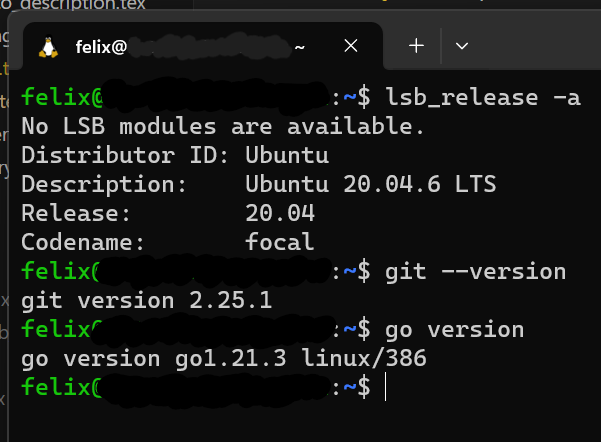
\includegraphics[width=0.8\textwidth]{figures/installation_screendump.png}
	\caption{Screendump showing the correct installation of the environment}
	\label{fig:screendump_installation}
\end{figure}

\section{Exercise CMGitLabUsage}

\subsection{Description of the M2Go Subgroup Structure}
The subgroup structure (figure \ref*{fig:screendump_subgroupStructure}) shows the Golang repository.
This repository consists out of three folder:
\begin{enumerate}
    \item BasicGoProgram/HelloWorld
    \item CarRental
    \item CarRentalCLI
\end{enumerate}
Further more there is the .gitignore file and the README.md file.

\begin{figure}[h]
    \centering
    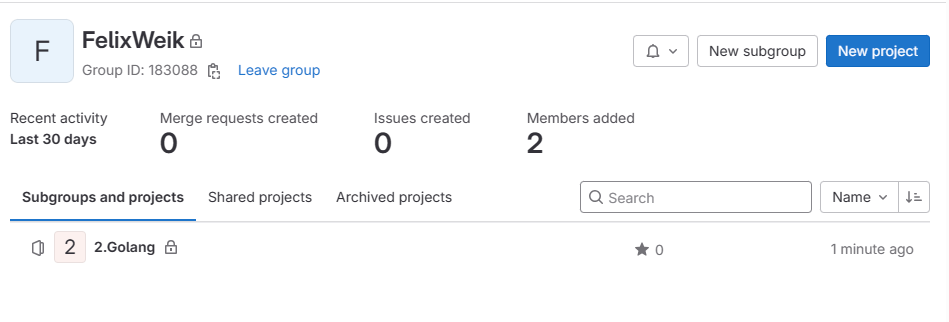
\includegraphics[width=0.8\textwidth]{figures/goLang/golang_personalSubgroupStructure.png}
    \caption{Screendump showing the subgroup structure}
    \label{fig:screendump_subgroupStructure}
\end{figure}

\subsection{Repository Cloning Steps}
To clone the repository, the following steps are required:
\begin{enumerate}
    \item Create a Personal Access Token (PAT) on GitLab by going to your profile settings and then to Access Tokens
    \item Save the PAT in a safe place
    \item Go to the repository and copy the HTTPS clone URL
    \item Open the WSL2 terminal and navigate to the folder where you want to clone the repository, in my case \texttt{/home/felix/WASA\_M2Go}
    \item Download the repository by running the following command in the terminal: \texttt{git clone <HTTPS clone URL>}
\end{enumerate}

\subsection{First Commit}
After changing the placeholder text in the README.md file, the first commit is done by using the graphical features Visual Studio Code offers.
The commit message (figure \ref*{fig:screendump_readmeCommitMessage}) is the following: \texttt{Update author and supervisor in README.md}.
After committing the changes, the changes are pushed to the remote repository, which then become visible on GitLab (figure \ref*{fig:screendump_readme}).

\begin{figure}[h]
    \centering
    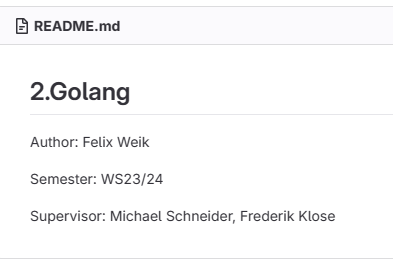
\includegraphics[width=0.5\textwidth]{figures/goLang/golang_screendumpReadme.png}
    \caption{Screendump showing the updated README.md file}
    \label{fig:screendump_readme}
\end{figure}

\begin{figure}[h]
    \centering
    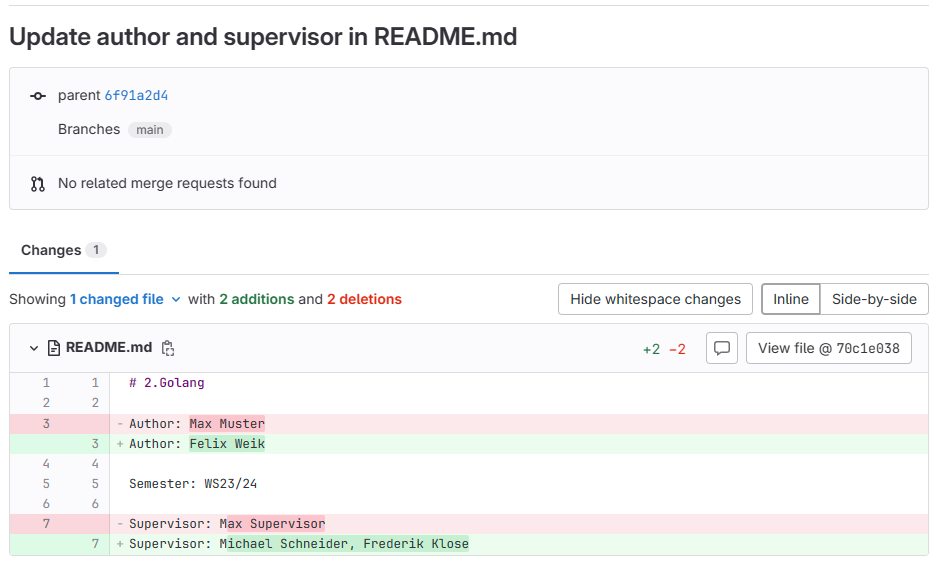
\includegraphics[width=0.8\textwidth]{figures/goLang/golang_screendumpReadmeCommit.png}
    \caption{Screendump showing commit message and the changed files}
    \label{fig:screendump_readmeCommitMessage}
\end{figure}

\section{Basic Hello World Program}
\subsection{Run Hello World}
After following the instruction in Mic-Con, the code is executed by running \texttt{go run main.go} in the terminal.
The code was executed twice: The first time the given code was executed leading to the output shown in figure \ref{fig:screendump_helloWorld_basicExecution}.
The second time the code was executed with different text, which can be seen in figure \ref{fig:screendump_helloWorld_differentText}.

\begin{figure} [h]
    \centering
    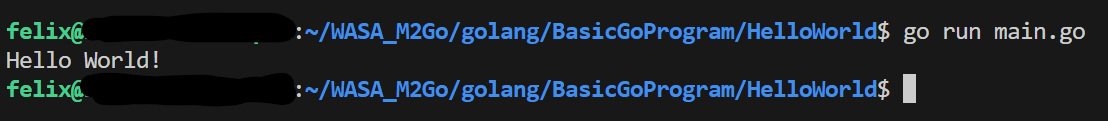
\includegraphics[width=0.8\textwidth]{figures/goLang/helloWorld/golang_helloWorld_basicExecution.png}
    \caption{Screendump showing the basic execution of the Hello World program}
    \label{fig:screendump_helloWorld_basicExecution}
\end{figure}

\begin{figure}[h]
    \centering
    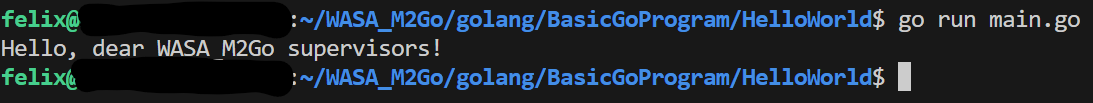
\includegraphics[width=0.8\textwidth]{figures/goLang/helloWorld/golang_helloWorld_ExecutionDifferentText.png}
    \caption{Screendump showing the execution of the Hello World program with different text}
    \label{fig:screendump_helloWorld_differentText}
\end{figure}

\subsection{Code Explanation}
\begin{lstlisting}[language=Golang]
    // main.go 
    // Author: Felix Weik

    package main    // package declaration: every executable belongs to the main package
                    // by declaring this package, a executable file is produced after compliation
    
    import "fmt"    // import the fmt package, a standard library package 
                    // implementing formatted I/O functions
                    // after import, one can use the functions of the imported package

    func main() {   // declares the function main, which is the 
                    // entry point of the program
        fmt.Println("Hello, World!")    // call the Println function 
                                        // of the fmt package; Println prints 
                                        // the given text to the standard output
    }               // end of the main function
\end{lstlisting}

